% Template for ICASSP-2016 paper; to be used with:
%          spconf.sty  - ICASSP/ICIP LaTeX style file, and
%          IEEEbib.bst - IEEE bibliography style file.
% --------------------------------------------------------------------------
\documentclass{article}
\usepackage{spconf,amsmath,graphicx}
\usepackage{amssymb}
\usepackage{mathrsfs}
\usepackage{epstopdf}
\usepackage{algorithmic}
\usepackage{algorithm}
\usepackage{subfigure}
\usepackage{multicol}
\usepackage{multirow}
\usepackage{url}

\renewcommand{\algorithmicrequire}{\textbf{Input:}}
\renewcommand{\algorithmicensure}{\textbf{Output:}}
% Example definitions.
% --------------------
\def\x{{\mathbf x}}
\def\L{{\cal L}}
\def\eg{\emph{e.g.}}
\def\ie{\emph{i.e.}}
\def\etal{\emph{et al.}}
\def\etc{\emph{etc.}}

% Title.
% ------
\title{Multiple Instance Hybrid Estimator for Learning Target Signatures}
%
% Single address.
% ---------------
\name{Changzhe Jiao and Alina Zare\thanks{This material is based upon work supported by the National Science Foundation under Grant IIS-1350078-CAREER: Supervised Learning for Incomplete and Uncertain Data.}}
\address{ Electrical and Computer Engineering, University of Missouri\\ Electrical and Computer Engineering, University of Florida}
%
% For example:
% ------------
%\address{School\\
%	Department\\
%	Address}
%
% Two addresses (uncomment and modify for two-address case).
% ----------------------------------------------------------
%\twoauthors
%  {A. Author-one, B. Author-two\sthanks{Thanks to XYZ agency for funding.}}
%	{School A-B\\
%	Department A-B\\
%	Address A-B}
%  {C. Author-three, D. Author-four\sthanks{The fourth author performed the work
%	while at ...}}
%	{School C-D\\
%	Department C-D\\
%	Address C-D}
%
\begin{document}
	%\ninept
	%
	\maketitle
	%
	\begin{abstract}
	Signature based detectors applied to hyperspectral target detection task rely on knowing the specific target signature in advance. However, in many cases, obtaining such target signature is difficult or impossible. Further more, target signature obtained from laboratory measurement or manual selection from the imagery does not capture the discriminative features of target class. This paper proposed an approach for learning target signature from imprecise labeling information of the targets. The proposed approach maximizes the response of the hybrid detector under a multiple instance framework and estimates a set of discriminative target concepts. After learning target signatures, any signature based detector could be applied for target detection on test data. Both simulated and real hyperspectral target detection experiments were conducted. 
		
	\end{abstract}
	%
	\begin{keywords}
		target detection, concept learning, hyperspectral, multiple instance.
	\end{keywords}
	%
	\section{Introduction}
	\label{sec:intro}
	The wealth of spectral information in hyperspectral imagery provides for the ability to perform sub-pixel target detection.   In statistical target detection methods, the target and background signals are modeled as random variables distributed according to some respective underlying distribution.  The detection problem can then be posed as a binary hypothesis test with two competing hypotheses: target absent ($\boldsymbol{H}_0$) or target present ($\boldsymbol{H}_1$) and a detector can be designed using the generalized likelihood ratio test (GLRT) approach.% \cite{Kay:1993,manolakis2014detection, nasrabadi2014hyperspectral}. 
	
	
	For detector based hyperspectral target detection, the problem is searching for a known signature within a hyperspectral scene. These target detection algorithms rely on an accurate  spectral signature for the target material to be known in advance. Ideally, the target spectral signature need to be fully characterized prior to application of a target detection algorithm. However, in a number of scenarios, obtaining an effective target signature is often a challenging problem.  For instance, an analyst or agent on the ground may only know approximate locations of some possibly sub-pixel targets identified by GPS coordinates (as ground truth information). Manually picking target signature from the imagery would be difficult and mixed with background material. Furthermore, spectral signatures obtained from a spectral library or collected using laboratory instruments do not account for variation due to environmental or atmospheric conditions.
	
	In this paper, we continue to investigate learning target signature from imprecisely labeled hyperspectral imagery, \ie, model the hyperspectral target endmember extraction task as a multiple instance concept learning problem. In multiple instance learning (MIL)  \cite{Dietterich:1997} problems, training data is grouped into bags instead of individually labeled. A positive bag must contain at least one true positive (target) data and negative bags are composed entirely negative data. Multiple instance concept learning is a branch of MIL that aims to learn one or a set of concept to describe the target category. The Diversity Density (DD) \cite{Maron:1998} tries to learn a concept for the positive class that is close to the intersection of positive bags and far always from every negative instance, \ie, an area preserves both high density of positive points and low density of negative points, called diversity density. The expectation maximization version of DD (EM-DD) \cite{Zhang:2002} adds a instance selection step in order to improve the convergence of DD. EM-DD selects only one instance per bag as the representative of the labeled bags then performs a quasi-newton optimization on the single-instance DD problem. 
	
	Some previous methods for hyperspectral target spectrum estimation given a MIL framework was proposed in \cite{Zare:2015fumi, zare2016miace}. \cite{Zare:2015fumi} combines all positive bags into one bigger positive bag and learns target signature from the reconstruction error, thus loses some bag-level labeling information. \cite{zare2016miace} maximizes the response of some matched filters and dose not assume a mixing model, thus may fail on some highly mixed detection problems. The proposed method overcomes the aforementioned drawbacks by maximizing the response of the hybrid detector (HD) \cite{Broadwater:2007} under a generalized mean framework.
	

	\section{Multiple Instance Hybrid Estimator}
	\label{sec:MIHE}
	
	Without loss of generality, let $\mathbf{X}=\left[\mathbf{x}_1,\cdots,\mathbf{x}_N\right]\in\mathbb{R}^{d\times N}$ be training data where $d$ is the dimensionality of an instance, $\mathbf{x}_j$, and $N$ is the total number of training instances. The data is grouped into $K$ \textit{bags},  $\mathbf{B} = \left\{ \mathbf{B}_1, \ldots, \mathbf{B}_K\right\}$, with associated binary bag-level labels, $L = \left\{L_1, \ldots, L_K\right\}$ where $L_i \in \left\{ 0, 1\right\}$; $n_i$ is the number of instances in bag $\mathbf{B}_i$ and $\mathbf{x}_{ij} \in \mathbf{B}_i$ denotes the $j^{th}$ instance in bag $\mathbf{B}_i$ with instance-level label $l_{ij}\in\left\{ 0, 1\right\}$. When the label on certain bag or instance matters,  it will be referred as positive bag $\mathbf{B}_i^+$ with bag level label $L_i^+$ containing instances $\mathbf{x}_{ij}^+$ with instance-level labels $l_{ij}^+, j=1,\cdots, n_i^+$, where $n_i^+$ is the number of instances in positive bag $\mathbf{B}_i^+$. Similarly, $\mathbf{B}_i^-,\: L_i^-,\: \mathbf{x}_{ij}^-,\: l_{ij}^-$ and $n_i^-$ represent a negative bag, label for this negative bag, the $j$th instance in this bag, label for the $j$th instance and total number of instances in this bag.  The number of positive and negative bags are denoted as $K^+$ and $K^-$, $N^+$ and $N^-$ represent the total number of positive and negative instances, respectively. Thus $N=N^++N^-=\sum_{i=1}^{K^+}n_i^++\sum_{i=1}^{K^-}n_i^-$ and $\mathbf{B}^+$,  $\mathbf{B}^-$ represent the union of all positive instances and negative instances, respectively.
	
	The proposed multiple instance hybrid estimator (MI-HE) starts from the bag-level likelihood measurement and wants to maximizes the probability of given bags,
	\begin{equation}
	J=\prod_{i=1}^{K^+} \Pr(L_i^+=1|\mathbf{B}_i^+)\cdot \prod_{i=1}^{K^-}\Pr(L_i^-=0|\mathbf{B}_i^-).
	\label{eq:MIHD_bag_likelihood}
	\end{equation}
	%
	Since the MIL problem defines there must be at least one (could be more) positive instance in each positive bag and the negative bag must consist of all negative instances, we can transfer the probability of individual bag to the instances in each bag, shown as Eq. \eqref{eq:MIHD_inst_likelihood}. Specifically, the probability for a positive bag to be positive is substituted by the instance in this bag with highest ``positiveness'' and the probability for a negative bag to be negative is represented by the join probability of all instances in this bag to be negative. 
	\begin{small}
	\begin{equation}
	J=\prod_{i=1}^{K^+} \max_{j\in n_i^+}\Pr(\mathbf{x}_{ij}^+=+|\mathbf{B}_i^+)\cdot \prod_{i=1}^{K^-}\prod_{j=1}^{n_i^-}\Pr(\mathbf{x}_{ij}^-=-|\mathbf{x}_{ij}^-).
	\label{eq:MIHD_inst_likelihood}
	\end{equation}
	\end{small}

	Eq. \eqref{eq:MIHD_inst_likelihood} contains a $\max$ operation that is difficult to optimize numerically. Some algorithms in the literature \cite{Maron:1998, Zhang:2002} adopt a noisy-OR model instead of using $\max$. However, experimental results show that the noisy-OR model is highly non-smooth and needs to repeat with many different initializations (typically using every positive training instance) to avoid local optima. In the proposed approach, we adopt the generalized mean as an alternative of $\max$ operation,
	\begin{small}
	\begin{equation}
	J=\prod_{i=1}^{K^+} \left(\frac{1}{n_i^+}\sum_{j=1}^{n_i^+}\Pr(\mathbf{x}_{ij}^+=+|\mathbf{B}_i^+)^p\right)^{\frac{1}{p}}\cdot \prod_{i=1}^{K^-}\prod_{j=1}^{n_i^-}\Pr(\mathbf{x}_{ij}^-=-|\mathbf{x}_{ij}^-),
	\label{eq:MIHD_gen_mean}
	\end{equation}
	\end{small}
	where $p\in [-\infty, +\infty]$ is a real number controls the function approximately to be from $\min$ to $\max$. 
	
	Then taking negative logarithm and scaling the negative part of the likelihood function result in Eq. \eqref{eq:MIHD_neg_log}:
\begin{figure*}[!t]
	\begin{equation}
	-\ln J=-\sum_{i=1}^{K^+}\frac{1}{p}\ln \left(\frac{1}{n_i^+}\sum_{j=1}^{n_i^+}\Pr(\mathbf{x}_{ij}^+=+|\mathbf{B}_i^+)^p\right)-\rho \sum_{i=1}^{K^-}\sum_{j=1}^{n_i^-}\ln\Pr(\mathbf{x}_{ij}^-=-|\mathbf{x}_{ij}^-),
	\label{eq:MIHD_neg_log}
	\end{equation}
	\end{figure*}
	where the scaling factor $\rho$ is usually set to be smaller than one to control the influence of negative bags. 
	
	Similar to \cite{jiao2016ICPR}, here each instance is modeled as a sparse linear combination of target and/or background concepts $\mathbf{D}$, $\mathbf{x}_j\approx\mathbf{D}\boldsymbol{\alpha}_j$, where $\boldsymbol{\alpha}_j$ is the sparse vector of  weights for instance $\mathbf{x}_j$. Each positive bag contains at least one instance composed of some target:
	\begin{eqnarray}
	&&\text{if }L_i = 1,  \nonumber \exists \mathbf{x}_j \in \mathbf{B}_i^+ \text{ s.t. } \\
	&&\mathbf{x}_j = \sum_{t=1}^{T}\alpha_{jt}\mathbf{d}_t^+ + \sum_{k=1}^{M} \alpha_{jk}\mathbf{d}_{k}^-+\boldsymbol{\varepsilon}_{j}, \alpha_{jt} \ne 0,
	\label{eq:MIHD_model_pos}
	\end{eqnarray}
	where $\boldsymbol{\varepsilon}_j$ is a noise term. And a negatively labeled bag $\mathbf{B}_i^-$ should not contain any target:
	\begin{equation}
	\text{if }L_i = 0,  \forall \mathbf{x}_j \in \mathbf{B}_i^-, \mathbf{x}_j =  \sum_{k=1}^{M} \alpha_{jk}\mathbf{d}_{k}^-+\boldsymbol{\varepsilon}_{j}.
	\label{eq:MIHD_model_neg}
	\end{equation}
	
	Given the above data model, we introduce the hybrid detector to discriminate the probability for instances from positive bags to be positive. Specifically, the probability for $\mathbf{x}_{ij}^+$ in $\mathbf{B}_i^+$ is defined as: 
	\begin{equation}
	\Pr(\mathbf{x}_{ij}^+=+|\mathbf{D},\boldsymbol{\alpha}_{ij}^+,\boldsymbol{\alpha}_{ij}^{+b})=\exp\left(-\beta\frac{\|\mathbf{x}_{ij}^+-\mathbf{D}\boldsymbol{\alpha}_{ij}^+\|^2}{\|\mathbf{x}_{ij}^+-\mathbf{D}^-\boldsymbol{\alpha}_{ij}^{+b}\|^2}\right),
	\label{eq:MIHD_pos_inst_model}
	\end{equation}
	%
	where $\mathbf{D}=\begin{bmatrix}\mathbf{D}^+ & \mathbf{D}^-\end{bmatrix}\in\mathbb{R}^{d\times (T+M)}$, $\mathbf{D}^+ = \left[\mathbf{d}_{1}^+,\cdots,\mathbf{d}_{T}^+\right]$ is the set of $T$ target  concepts and $\mathbf{D}^- = \left[\mathbf{d}_{1}^-,\cdots,\mathbf{d}_{M}^-\right]$ is the set of $M$ background  concepts, $\beta$ is a scaling parameter;  $\boldsymbol{\alpha}_{ij}^{+}$ and $\boldsymbol{\alpha}_{ij}^{+b}$ are the sparse representation of $\mathbf{x}_{ij}^+$ given entire concept set $\mathbf{D}$ and background concept set $\mathbf{D}^-$, respectively. Specifically, solving the sparse representation $\boldsymbol{\alpha}$ given a dictionary set $\mathbf{D}$ is modeled as a Lasso problem \cite{tibshirani1996regression, chen2001atomic} shown in Eq. \eqref{eq:MIHD_lasso}:
	\begin{equation}
	\hat{\boldsymbol{\alpha}}=\arg\min\frac{1}{2}\|\mathbf{x}-\mathbf{D}\boldsymbol{\alpha}\|^2_2+\lambda\|\boldsymbol{\alpha}\|_1,
	\label{eq:MIHD_lasso}
	\end{equation}
	where $\lambda$ is a scaling vector to control the sparsity of $\boldsymbol{\alpha}$. Here we adopt the iterative shrinkage-thresholding algorithm (ISTA) \cite{daubechies2003iterative} for solving the sparse codes  $\boldsymbol{\alpha}$.
	
%	The definition of $\Pr(\mathbf{x}_{ij}^+=+|\mathbf{D},\boldsymbol{\alpha}_{ij}^+,\boldsymbol{\alpha}_{ij}^-)$ in \eqref{eq:MIHD_pos_inst_model} indicates if a point $\mathbf{x}_{ij}^+\in \mathbf{B}_i^+$ is a true positive point, it could not be well represented by only the non-target concepts, so the residual error approximated by the entire concepts, $\|\mathbf{r}_{ij}^+\|^2$, will be much smaller than that by the background concepts $\|\mathbf{r}_{ij}^{+b}\|^2$, thus $\Pr(\mathbf{x}_{ij}^+=+|\mathbf{D},\boldsymbol{\alpha}_{ij}^+,\boldsymbol{\alpha}_{ij}^{+b})=\exp\left(-\beta\frac{\|\mathbf{r}_{ij}^{+b}\|^2}{\|\mathbf{r}_{ij}^+\|^2}\right)\rightarrow 1$. Otherwise, if  $\mathbf{x}_{ij}^+\in \mathbf{B}_i^+$ is a false positive point, $\|\mathbf{r}_{ji}^+\|^2\approx \|\mathbf{r}_{ij}^{+b}\|^2$, thus $\Pr(\mathbf{x}_{ij}^+=+|\mathbf{D},\boldsymbol{\alpha}_{ij}^+,\boldsymbol{\alpha}_{ij}^{+b})=\exp\left(-\beta\frac{\|\mathbf{r}_{ij}^{+b}\|^2}{\|\mathbf{r}_{ij}^+\|^2}\rightarrow 0\right)$.
	
	For points from negative bags, following Eq. \eqref{eq:MIHD_model_neg}, we model the reconstruction error of points $\mathbf{x}_{ij}^- \in \mathbf{B}_i^+$ as a zero mean Gaussian distribution with unknown variance, shown as Eq. \eqref{eq:MIHD_neg_inst_model},
	\begin{equation}
	\Pr(\mathbf{x}_{ij}^-=-|\mathbf{D}^-,\boldsymbol{\alpha}_{ij}^-)=\exp\left(\|\mathbf{x}_{ij}^--\mathbf{D}^-\boldsymbol{\alpha}_{ij}^-\|^2\right),
	\label{eq:MIHD_neg_inst_model}
	\end{equation}
	%
	%
	where $\boldsymbol{\alpha}_{ij}^-$ is the sparse representation of $\mathbf{x}_{ij}^-$ given $\mathbf{D}^-$ and is solved by solving Eq. \eqref{eq:MIHD_lasso}. 
	
	The objective function \eqref{eq:MIHD_neg_log} is optimized by gradient descent with sparse coding shown in Alg. \ref{alg:MIHD}
	\begin{algorithm}
		\caption{MI-HE algorithm}
		\algsetup{indent=4em}
		\begin{algorithmic}[1] 
			\STATE Initialize $\mathbf{D}^0$, $iter = 0$
			\REPEAT
			\FOR{$t=1,\cdots,T$}
			\STATE Solving $\begin{small}\left\{\boldsymbol{\alpha}^+_i \right\}_{i=1}^{N}\end{small}$, $\begin{small}\left\{\boldsymbol{\alpha}^-_i \right\}_{i=1}^{N}\end{small}$ by ISTA
			\STATE Update  $\mathbf{d}_t$ by optimizing \eqref{eq:MIHD_neg_log} using gradient descent
			\STATE $\mathbf{d}_t\gets\frac{1}{\|\mathbf{d}_t\|_2}\mathbf{d}_t$
			\ENDFOR
			\FOR{$k=1,\cdots,M$}
			\STATE Solving  $\begin{small}\left\{\boldsymbol{\alpha}^+_i \right\}_{i=1}^{N}\end{small}$, $\begin{small}\left\{\boldsymbol{\alpha}^-_i \right\}_{i=1}^{N}\end{small}$ by ISTA
			\STATE Update  $\mathbf{d}_k$ by optimizing \eqref{eq:MIHD_neg_log} using gradient descent
			\STATE $\mathbf{d}_k\gets\frac{1}{\|\mathbf{d}_k\|_2}\mathbf{d}_k$
			\ENDFOR
			\STATE $iter \gets iter + 1$
			\UNTIL{Stopping criterion meets}
			\RETURN $\mathbf{D}$\\
		\end{algorithmic} 
		\label{alg:MIHD}
	\end{algorithm}
	
	
	
	\section{EXPERIMENTS}
	\label{sec:experiments}
	
	MI-HE was run on simulated data generated from four spectra selected from the ASTER spectral library \cite{aster:2009} shown in Fig. \ref{fig:constituent_endmembers}. Specifically, the Red Slate, Verde Antique, Phyllite and Pyroxenite spectra from the rock class with 211 bands and wavelengths ranging from $0.4 \mu$m to $2.5 \mu$m were used as endmembers to generate hyperspectral data. Red Slate was labeled as the target endmember. \cite{Zare:2015fumi} provides a precise description of how the simulated data was generated. 
	
	\begin{figure}
		\centering
		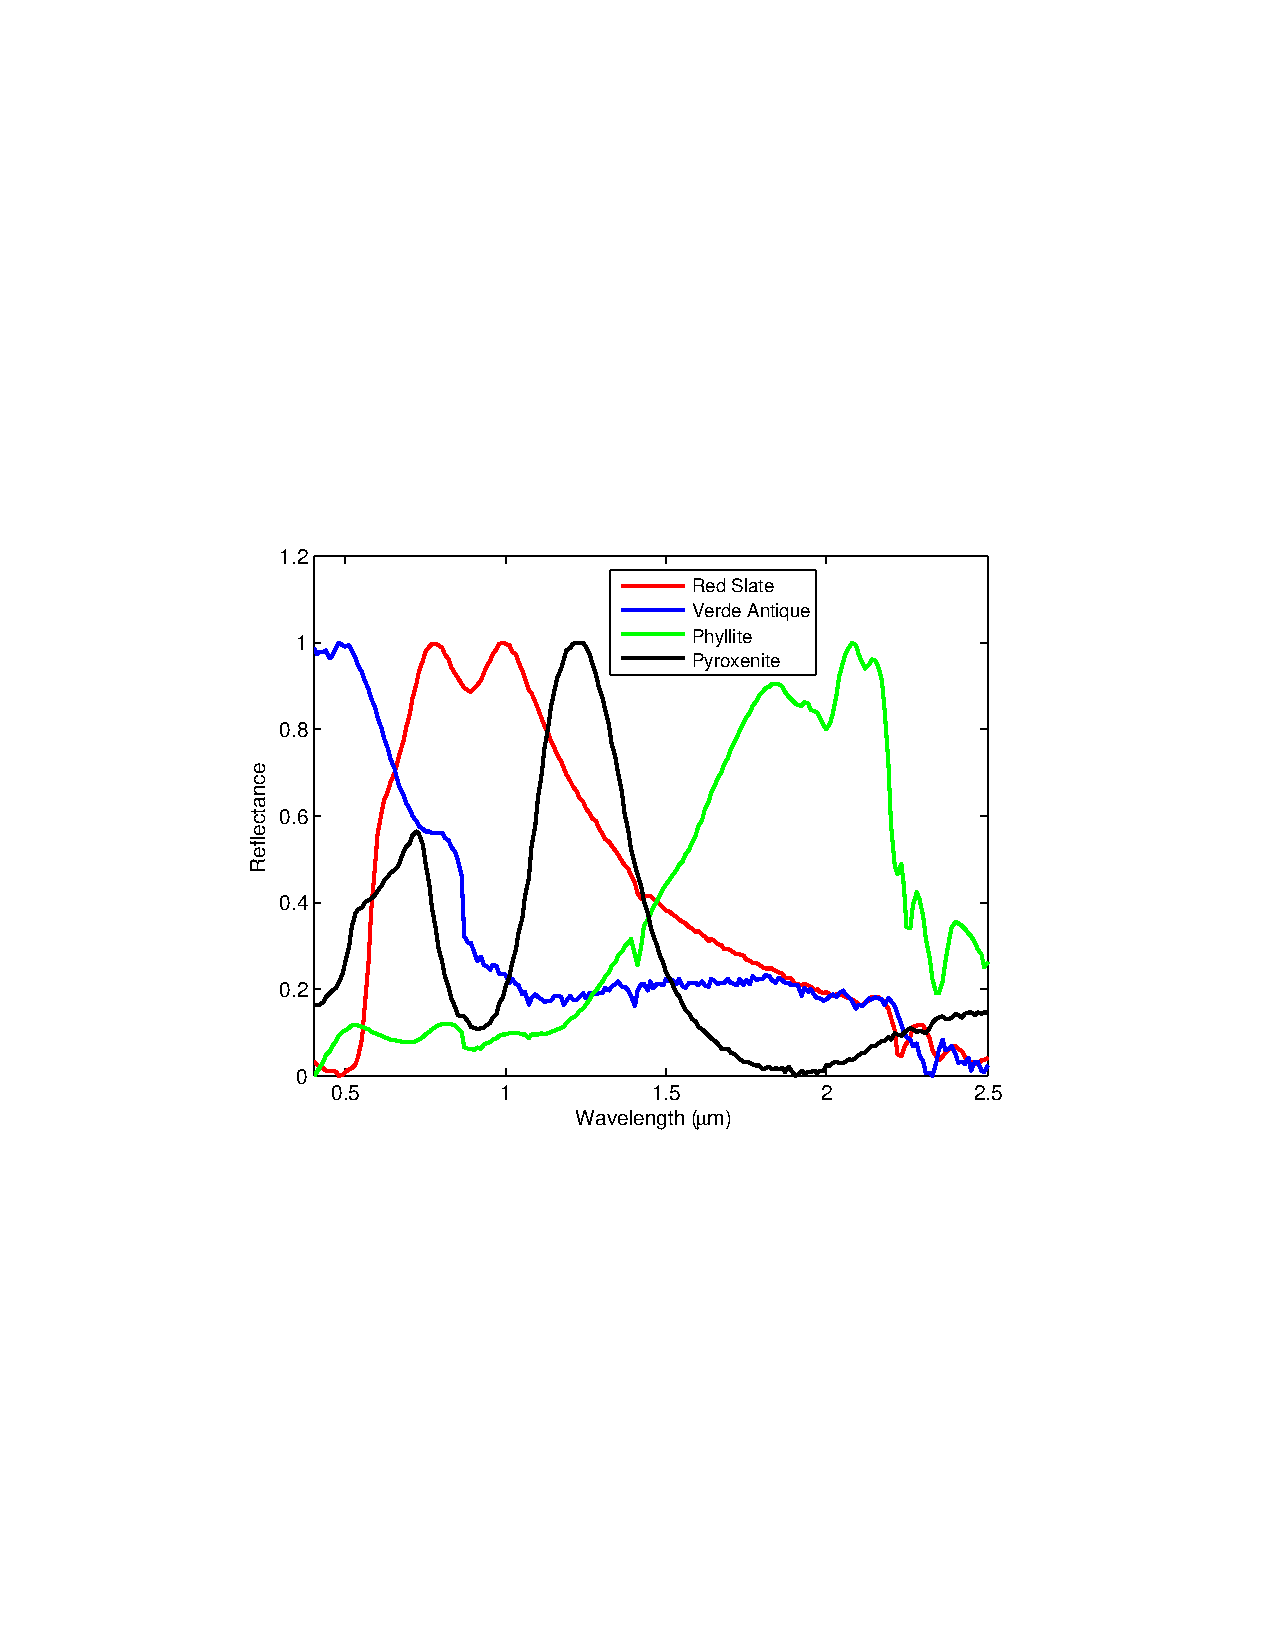
\includegraphics[width=6cm]{aster_endmembers_plot.pdf}
		\caption{Signatures from ASTER library used to generate simulated data \label{fig:constituent_endmembers} } 
	\end{figure}
	
	Three sets of highly-mixed noisy data with varied mean target proportion value ($p_{t\_mean}$) were generated, respectively. Specifically, this synthetic data has 15 positive and 5 negative bags with each bag has 500 points. If it is positively labeled, there are 100 target points with $p_{t\_mean}$ target proportion. The parameter $p_{t\_mean}$ that controls the mean target proportion value was set to 0.3, 0.5 and 0.7 respectively to get different level of target presence from weak to high. Gaussian white noise was added so that signal-to-noise ratio of the data was set to $30 dB$. What is different from the synthetic data in \cite{Zare:2015fumi} is there are only two background endmembers, Phyllite and Pyroxenite, involved in the negative bags; in the first 5 positive bags, target endmember Red Slate and all three background endmembers are presented; in the second 5 positive bags target endmember Red Slate and two background endmembers, Phyllite and Pyroxenite, are present; in the last 5 positive bags, only target endmember and one background endmember Pyroxenite are present. 
	
	As we mentioned before, $e$FUMI combines all positive bags into one big positive bags. Given the aforementioned synthetic data, theoretically $e$FUMI will confuse both Red Slate and Verde Antique as target concept since Verde Antique is missing in the training negative bags. However, the proposed MI-HE should be able to learn the target concept correctly since it aims to maximize the detection statistics of each positive bag. Fig. \ref{fig:sig_plot_toydata_ptmean03} shows the estimated target signature estimated by MI-HE and comparison algorithms $e$FUMI \cite{Zare:2015fumi} and EM-DD \cite{Zhang:2002}, where we can see that MI-HE is able to learn an exact target signature as groundtruth, but $e$FUMI mistakes Verde Antique as target concept and EM-DD learns one noisy and non-pure target signature. 
	
	
	For quantitative evaluation, receiver operating curves (ROC) from detection on testing data generated using the same method are shown in Fig. \ref{fig:rocs_toydata_ptmean03}. Tab. \ref{tab:AUC_toydata} shows the normalized area of probability of detection (PD) under the curve (NAUC) at false alarm rate (FAR) $1\times 10^{-3}$, where we can see proposed MI-HE outperforms the comparison algorithms $e$FUMI, EM-DD and mi-SVM \cite{andrews:2002}. For MI-HE and $e$FUMI, both detectors, structured-background adaptive coherence/cosine estimator (ACE) \cite{Kraut:1999, basener:2010clutter} and HD \cite{Broadwater:2007} were applied; for EM-DD, only ACE was applied since EM-DD does not learn a set of background concept simultaneously. The results reported are the median results over five runs of the algorithm on the same data.   
	
	
			
	\begin{figure}
		\begin{center}
			\subfigure[Estimated target spectra]{   
				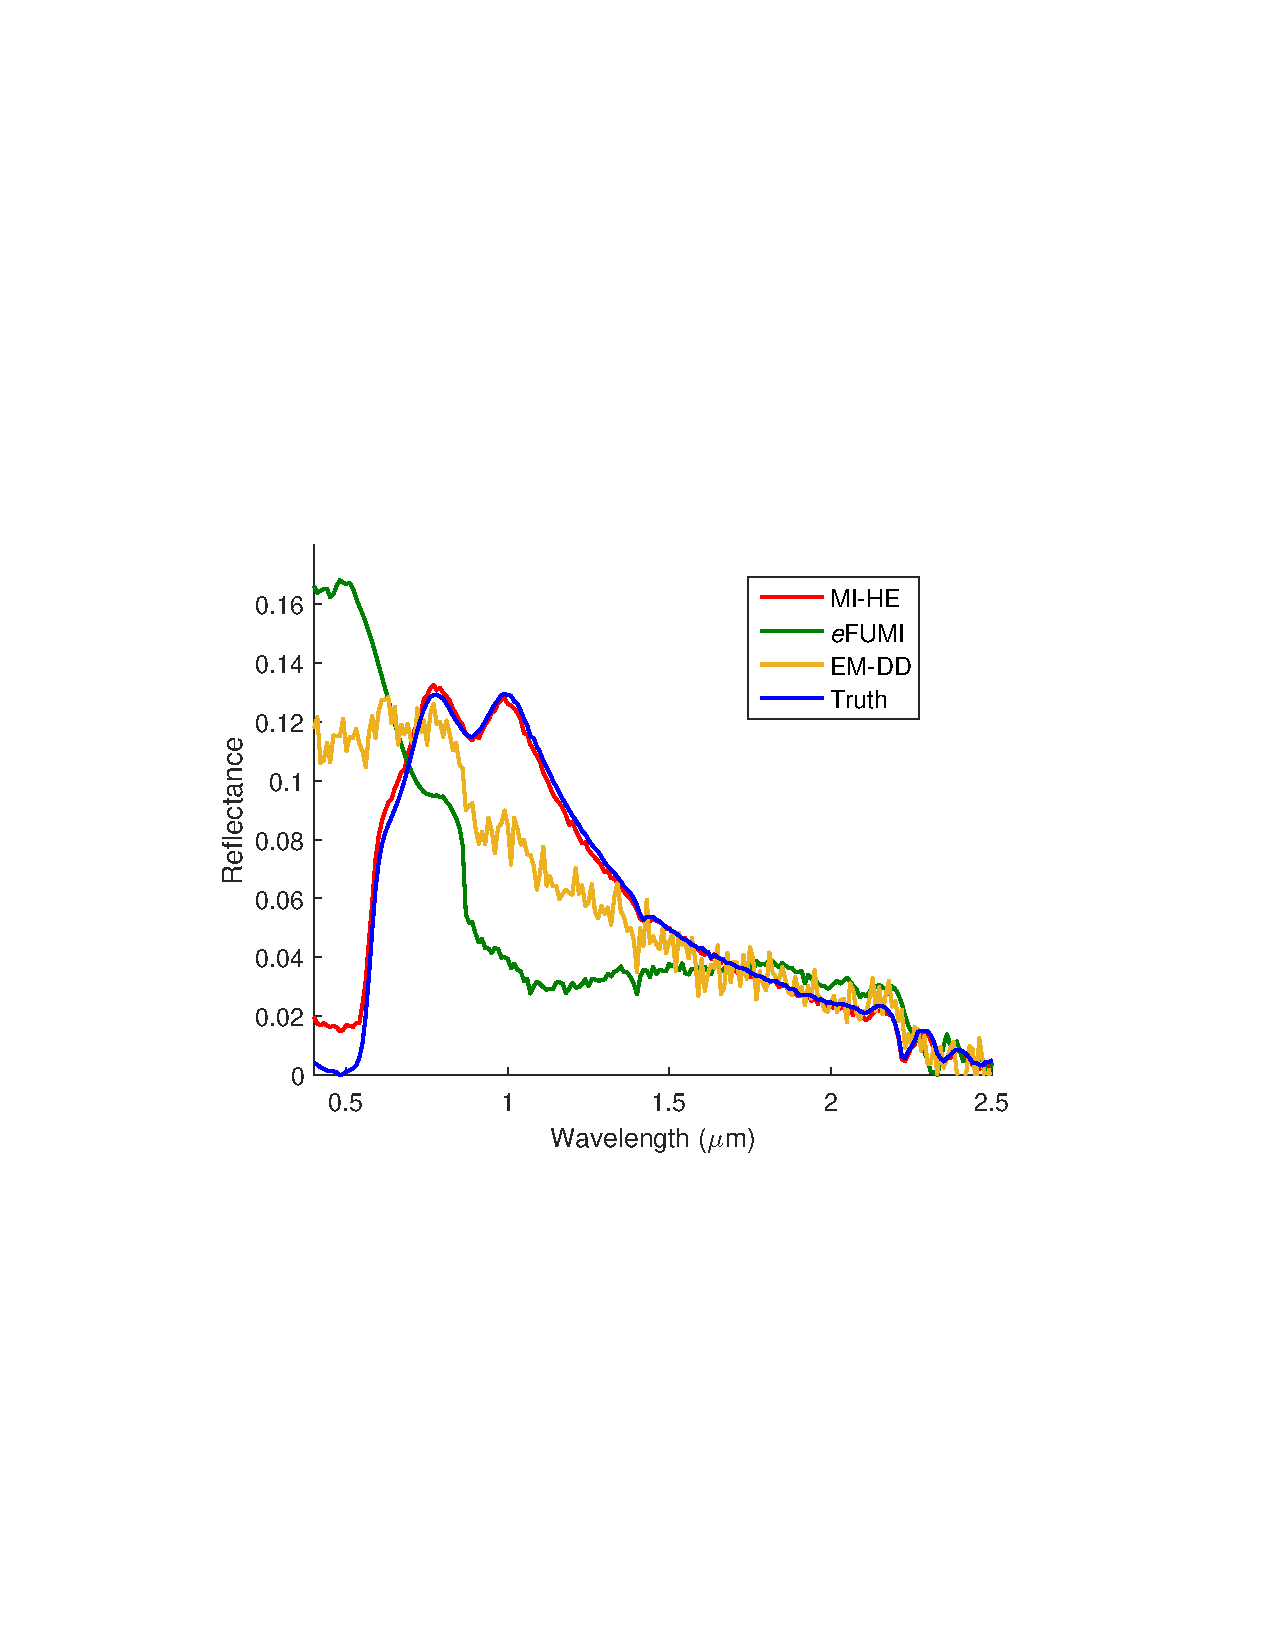
\includegraphics[width=7cm]{overlapbags_sigs_pt_mean_03.pdf} \label{fig:sig_plot_toydata_ptmean03}}
			\subfigure[ROC curves]{   
				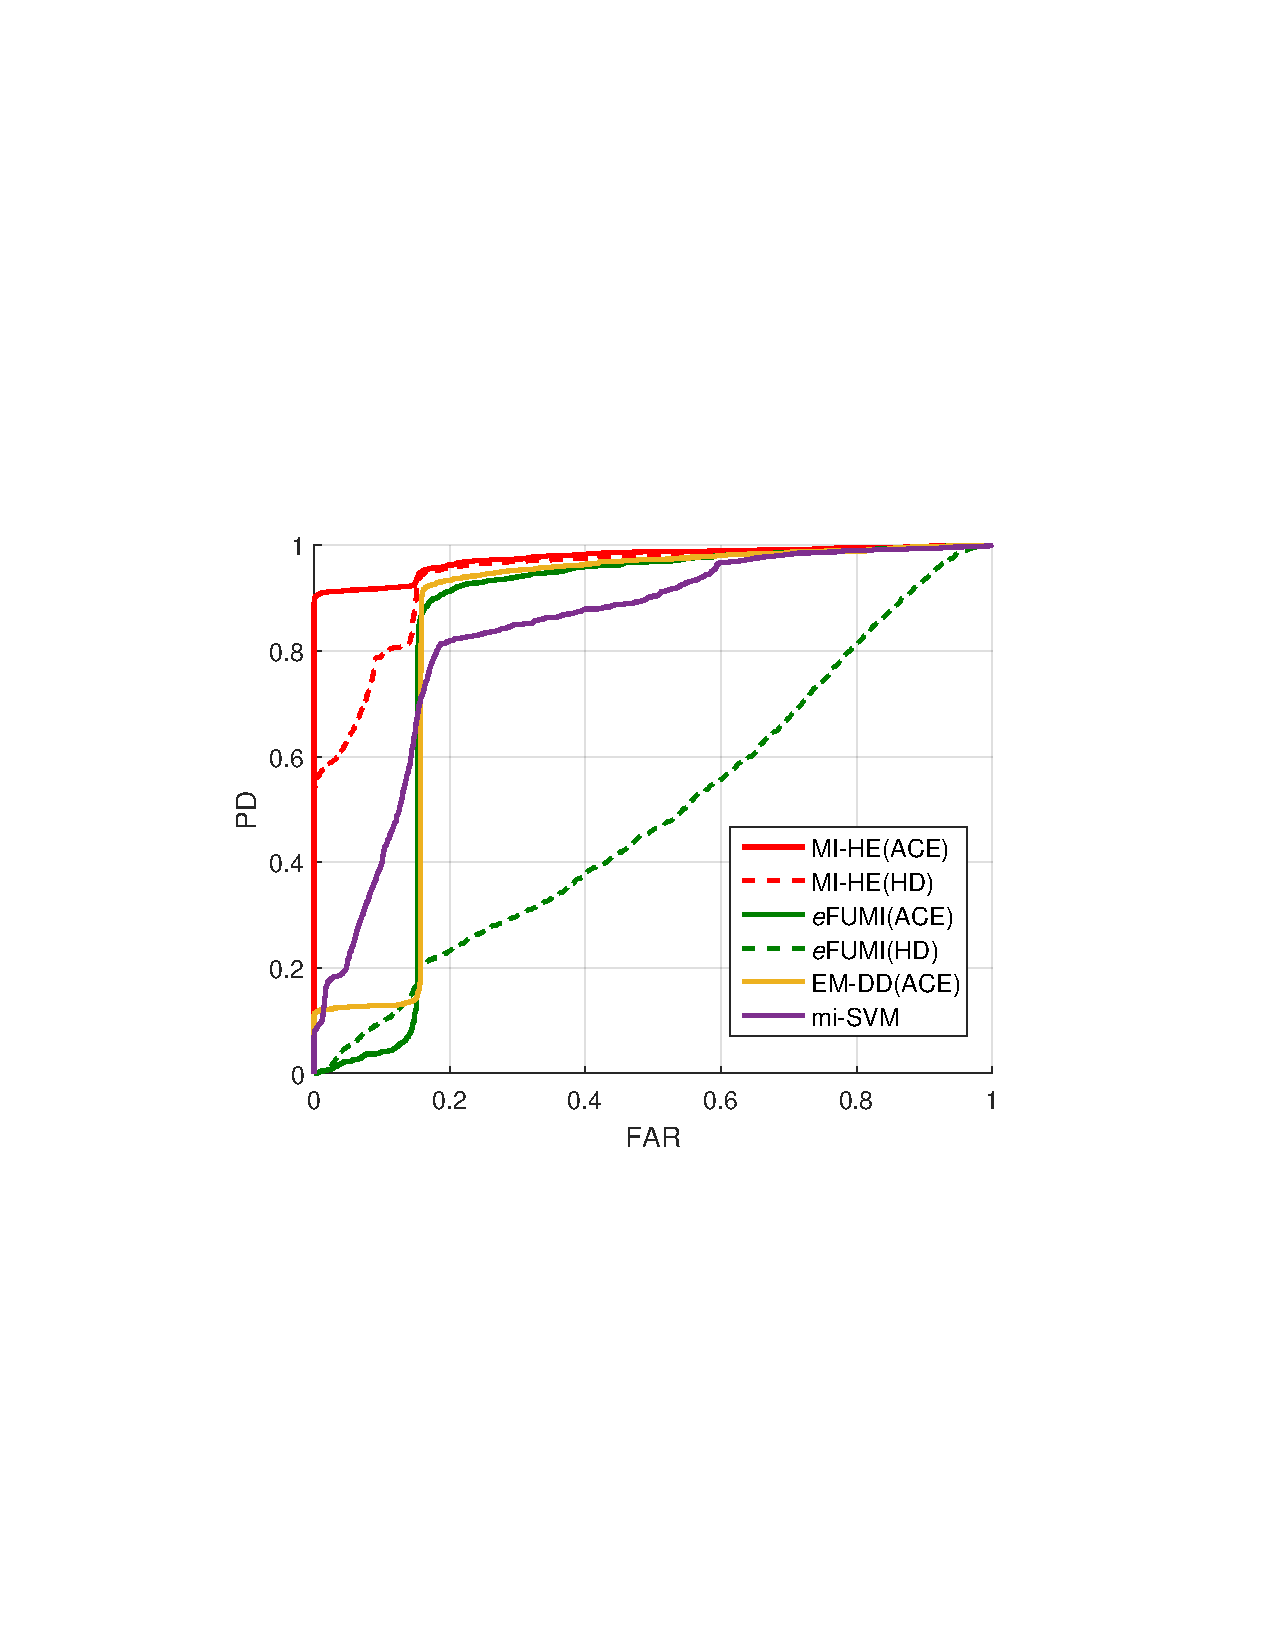
\includegraphics[width=7cm]{overlapbags_rocs_pt_mean_03.pdf} \label{fig:rocs_toydata_ptmean03}}
			\caption{Comparison of MI-HE, $e$FUMI, EM-DD and mi-SVM on synthetic data with mean target proportion 0.3}\label{fig:compare_tyodata_ptmean_03}
		\end{center}
	\end{figure}

\begin{table} 
	\begin{center}
		\caption{Simulated Hyperspectral Data Experiments. Results listed in Median NAUC over 5 Runs at FAR $=1\times10^{-3}$}\label{tab:AUC_toydata}
		\begin{tabular}{|c|c|c|c|}
			\hline
			\multirow{2}{*}{Algorithm} 	&  \multicolumn{3}{c|}{$P_{t\_mean}$} \\
			\cline{2-4}&{0.3}&{0.5}&{0.7}\\
			\hline\hline
			{MI-HE (HD)}      &   \underline{0.537}      &      \underline{0.670}              &   0.952     \\\hline
			{MI-HE (ACE)}     &      \textbf{0.895}      &      \textbf{0.978}     &   \textbf{0.998}    \\\hline
			{$e$FUMI (ACE)}  &      0.0                 &      0.0                &   0.0    \\\hline
			{$e$FUMI (HD)}   &      0.0                 &      0.0                &   0.0     \\\hline
			{EM-DD (ACE)}    &      0.113               &      {0.158}  &   \underline{0.986}    \\\hline
			{mi-SVM}         &      0.075               &      0.0              &   {0.0}    \\\hline
		\end{tabular}
	\end{center}
\end{table}

\begin{figure}
	\centering
	{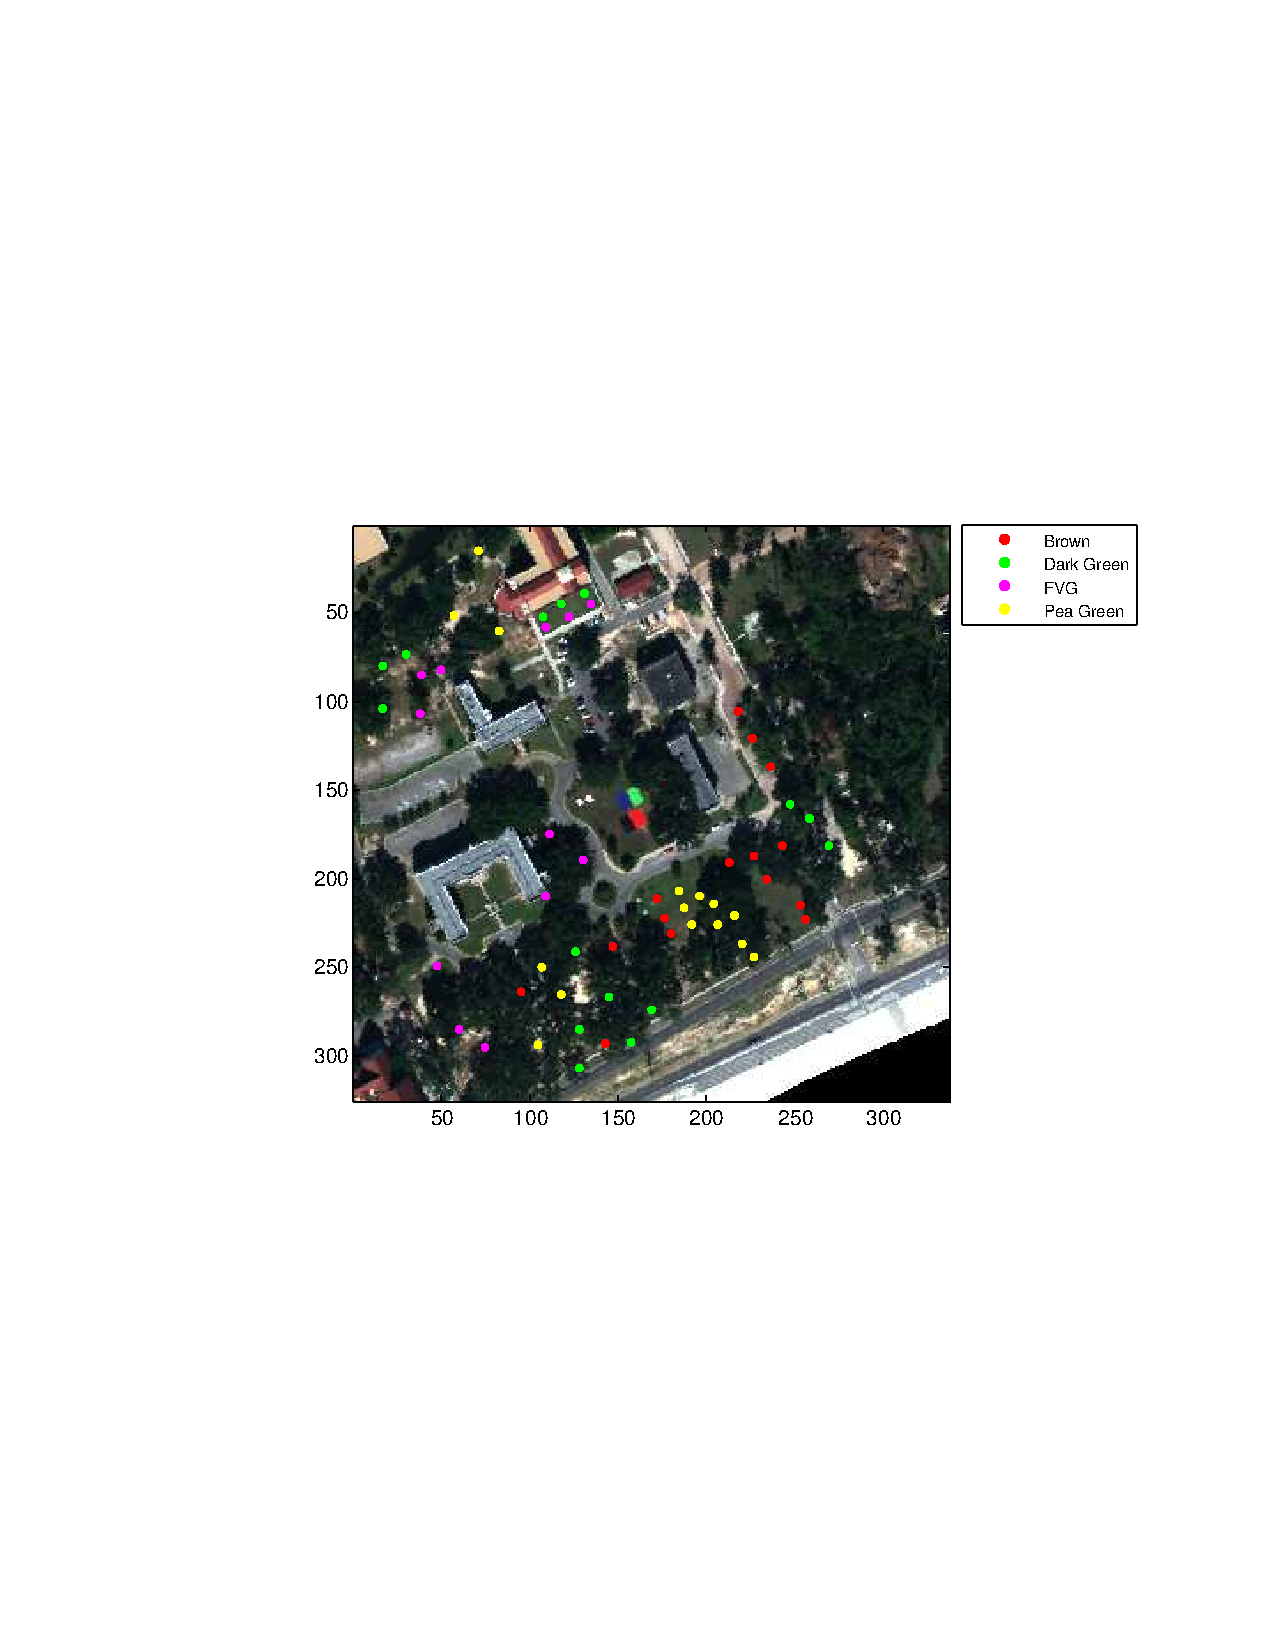
\includegraphics[width=7cm]{Fig_muufl.pdf}}
	\caption{MUUFL Gulfport data set RGB image and the 64 target locations}
	\label{fig:gulfport_rgb}
\end{figure}

\begin{table} 
	\begin{scriptsize}
		\begin{center}
			\caption{Gulfport Brown Detection. Results listed in Median NAUC over 5 Runs at FAR $=1\times10^{-3}$}\label{tab:AUC_gulfport}
			\begin{tabular}{|c|c|c|}
				\hline
				{Algorithm} 	&  {Train: Flight 1, Test: Flight 3}& {Train: Flight 3, Test: Flight 1} \\
				\hline\hline
				{MI-HE (HD)}&      \textbf{0.552}     &  \textbf{0.792}         \\\hline
				{MI-HE (ACE)}&          \underline{0.442}         &     {0.699}                       \\\hline
				{$e$FUMI (ACE)}&       0.437         &      0.746                    \\\hline
				{$e$FUMI (HD)}&        0.417         &      \underline{0.765}                     \\\hline
				{EM-DD (ACE)}&        {0.420}   &     {0.749}                      \\\hline
				{mi-SVM}&        0.353         &   0.333      \\\hline
			\end{tabular}
		\end{center}
	\end{scriptsize}
\end{table}


  For experiments on real hyperspectral target detection data, the MUUFL Gulfport Hyperspectral data set was used.  This data set was collected over the University of Southern Mississippi-Gulfpark Campus and contains $325\times337$ pixels with 72 bands corresponding to wavelengths from $367.7 nm$ to $1043.4 nm$ at a $9.5-9.6 nm$ spectral sampling interval. The spatial resolution is 1 m. \cite{gader:2013} provides more detailed information about the data. Two flights over the area from this data (Gulfport Campus Flight 1 and Gulfport Campus Flight 3) were selected as cross-validated training and testing data. Throughout the scene, there are 64 emplaced man-made targets shown in Fig. \ref{fig:gulfport_rgb}. The targets are cloth panels of four different colors: Brown (15 examples), Dark Green (15 examples), Faux Vineyard Green (FVG) (12 examples) and Pea Green (15 examples). We take Brown as our target type and for each target in the training flight, a $5\times5$ rectangular region around each ground truth point for each target were labeled as positive bags to account the drift coming from GPS groundtruthing. 




For the quantitative analysis of the estimated brown signatures, the NAUCs  at FAR $1\times 10^{-3}$ were computed and were shown in Tab. \ref{tab:AUC_gulfport}, where the proposed MI-HE combined with HD preserves the best detection performance. Results reported are the median results over five runs.  



%\begin{figure}
%	\begin{center}
%		\subfigure[Estimated target spectra]{   
%			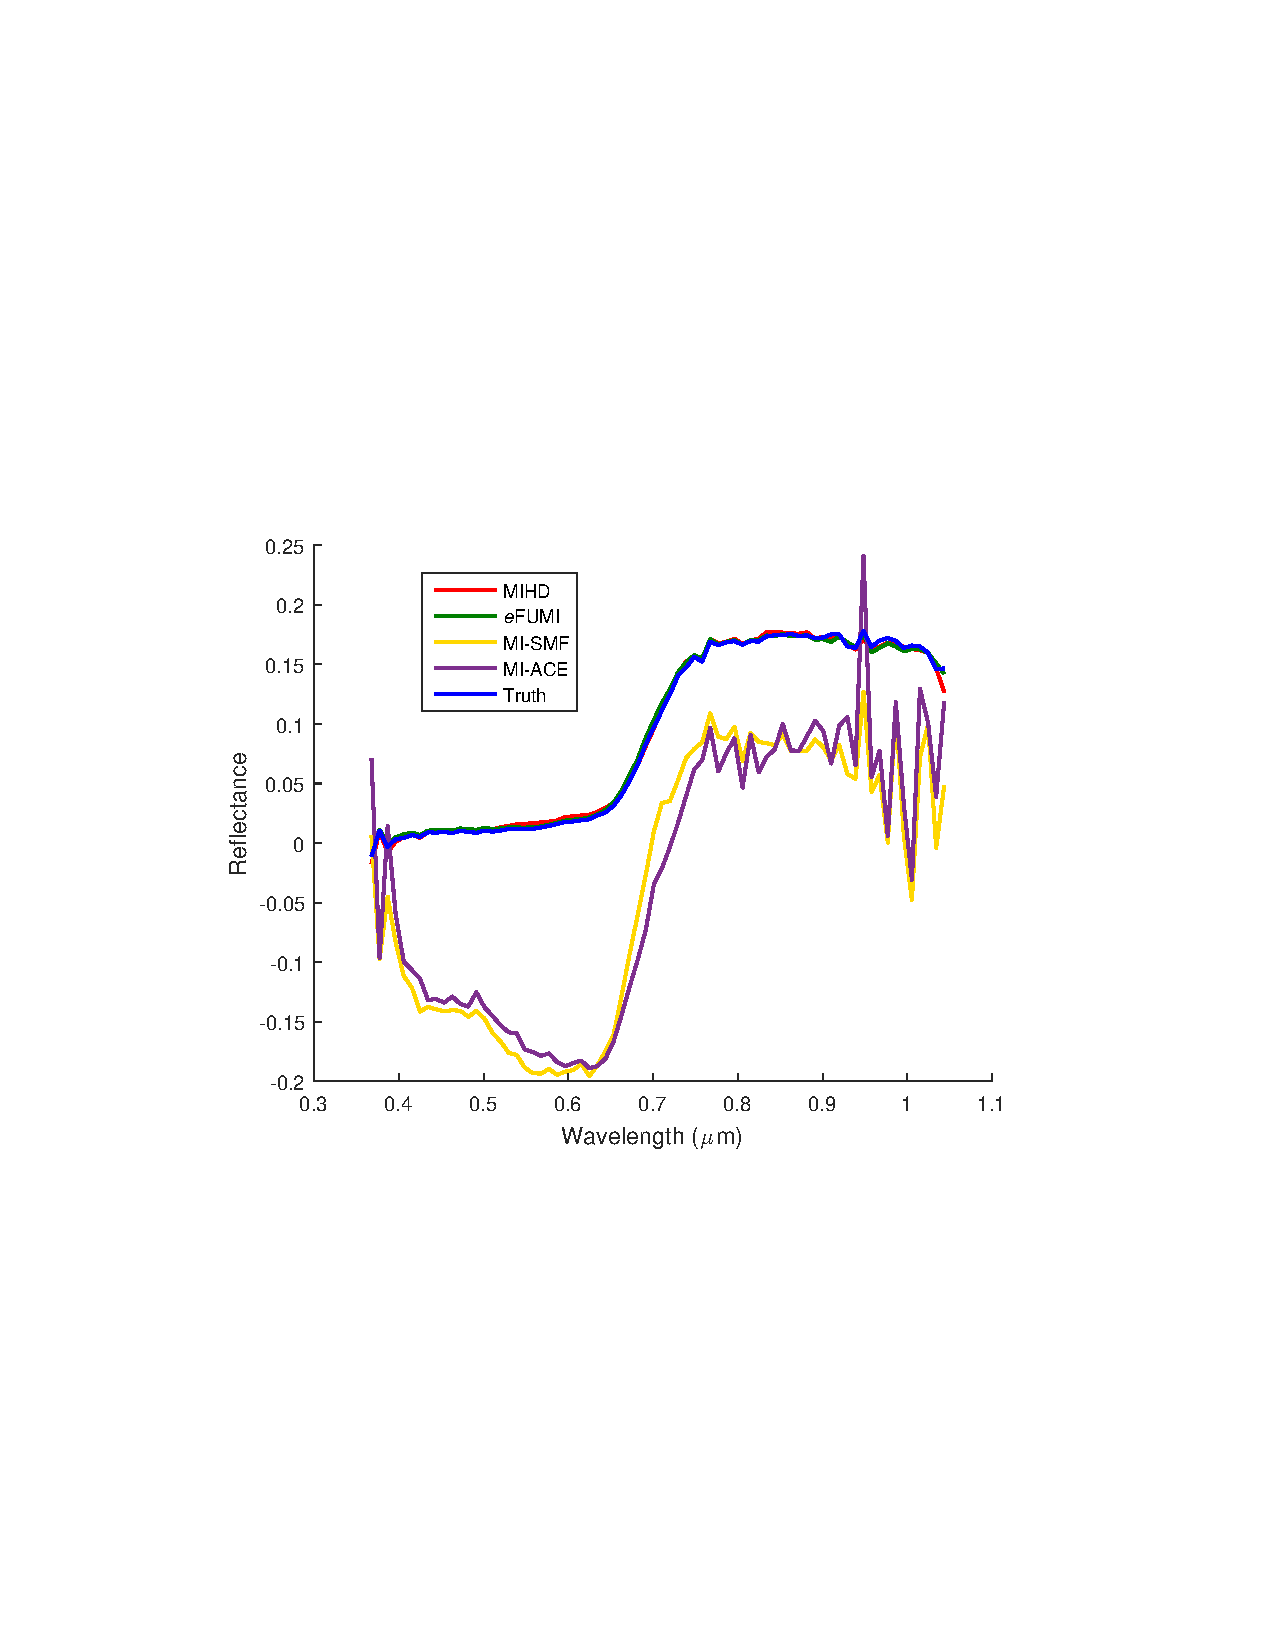
\includegraphics[width=4cm]{gulfport_sigs_brown_train1_test3.pdf} \label{fig:sig_plot_gulfport_brown_train1_test3}}
%		\subfigure[ROC curves]{   
%			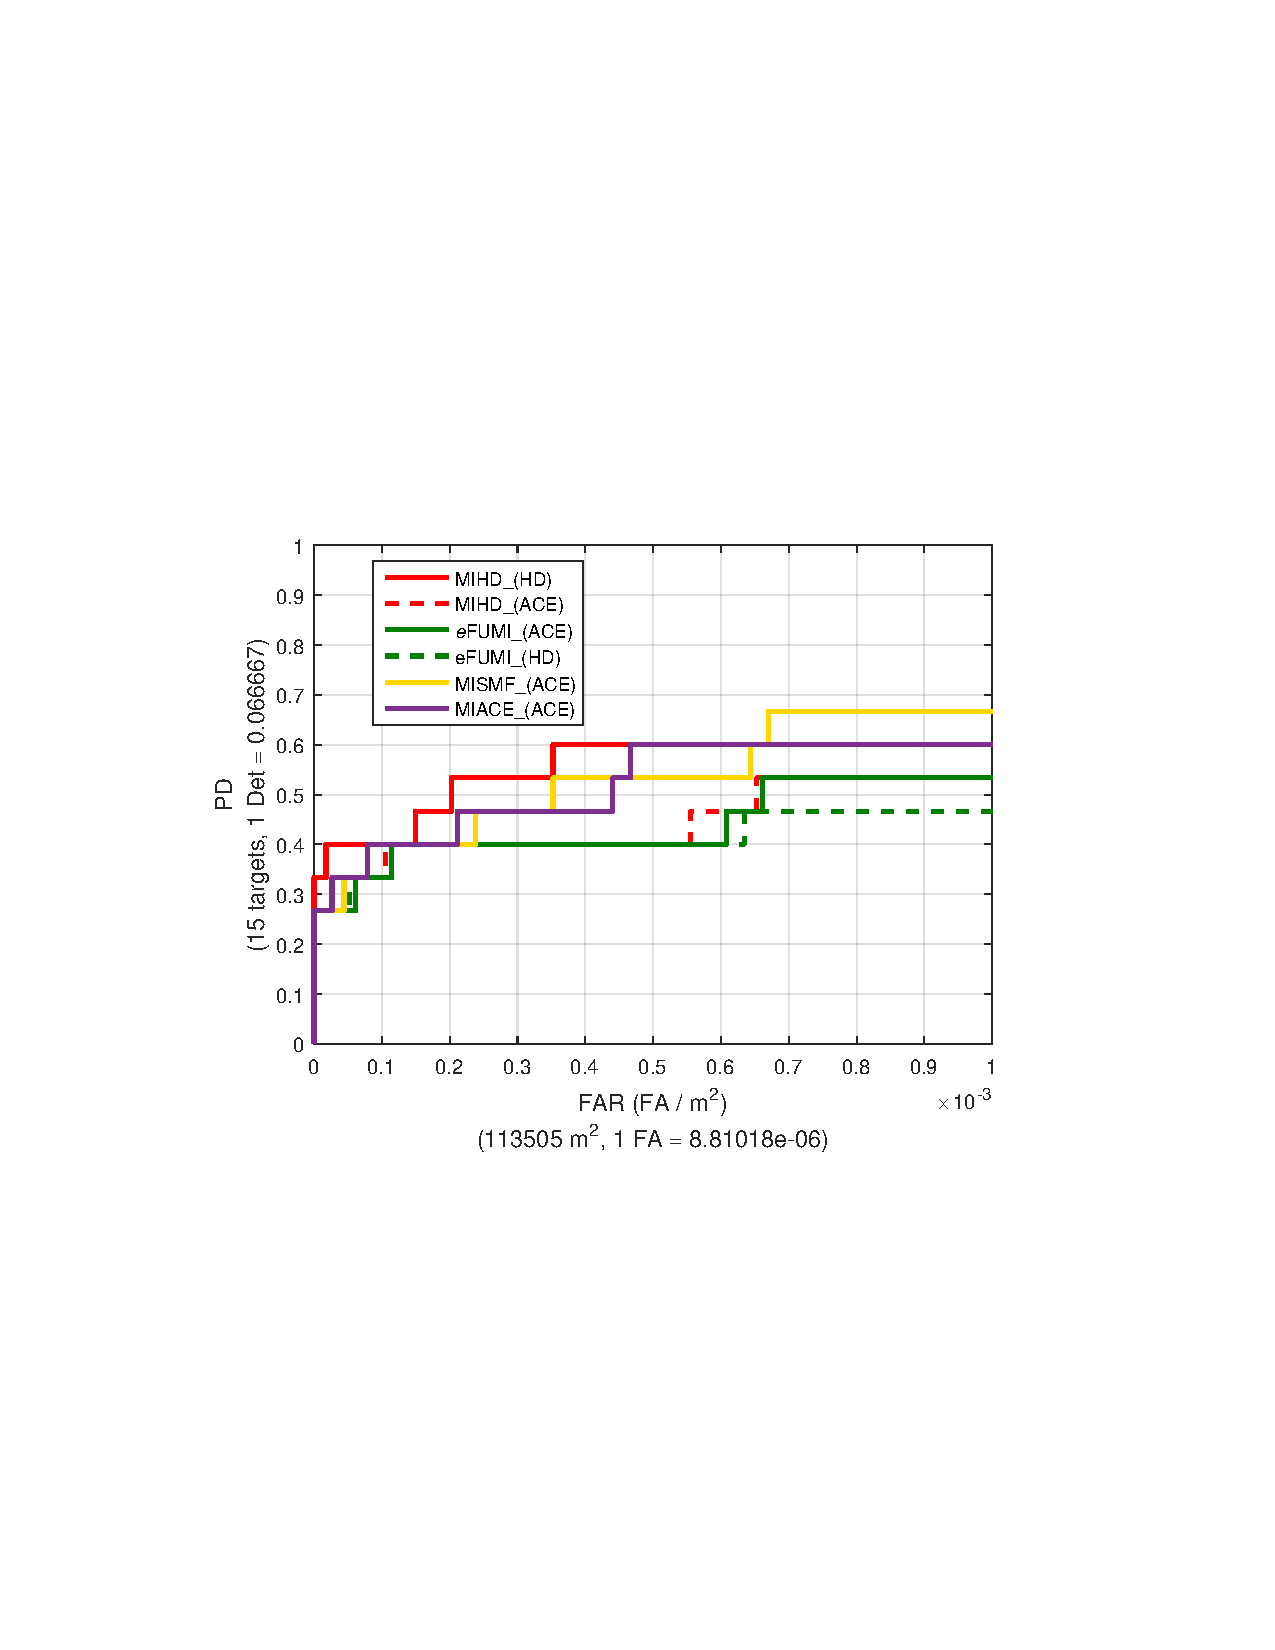
\includegraphics[width=4cm]{gulfport_rocs_brown_train1_test3.pdf} \label{fig:rocs_gulfport_brown_train1_test3}}
%		\caption{Comparison of MI-HE, $e$FUMI, EM-DD and mi-SVM on Gulfport Brown, training on flight 1 testing on flight 3}\label{fig:compare_gulfport_brown_train1_test3}
%	\end{center}
%\end{figure}
%
%\begin{figure}
%	\begin{center}
%		\subfigure[Estimated target spectra]{   
%			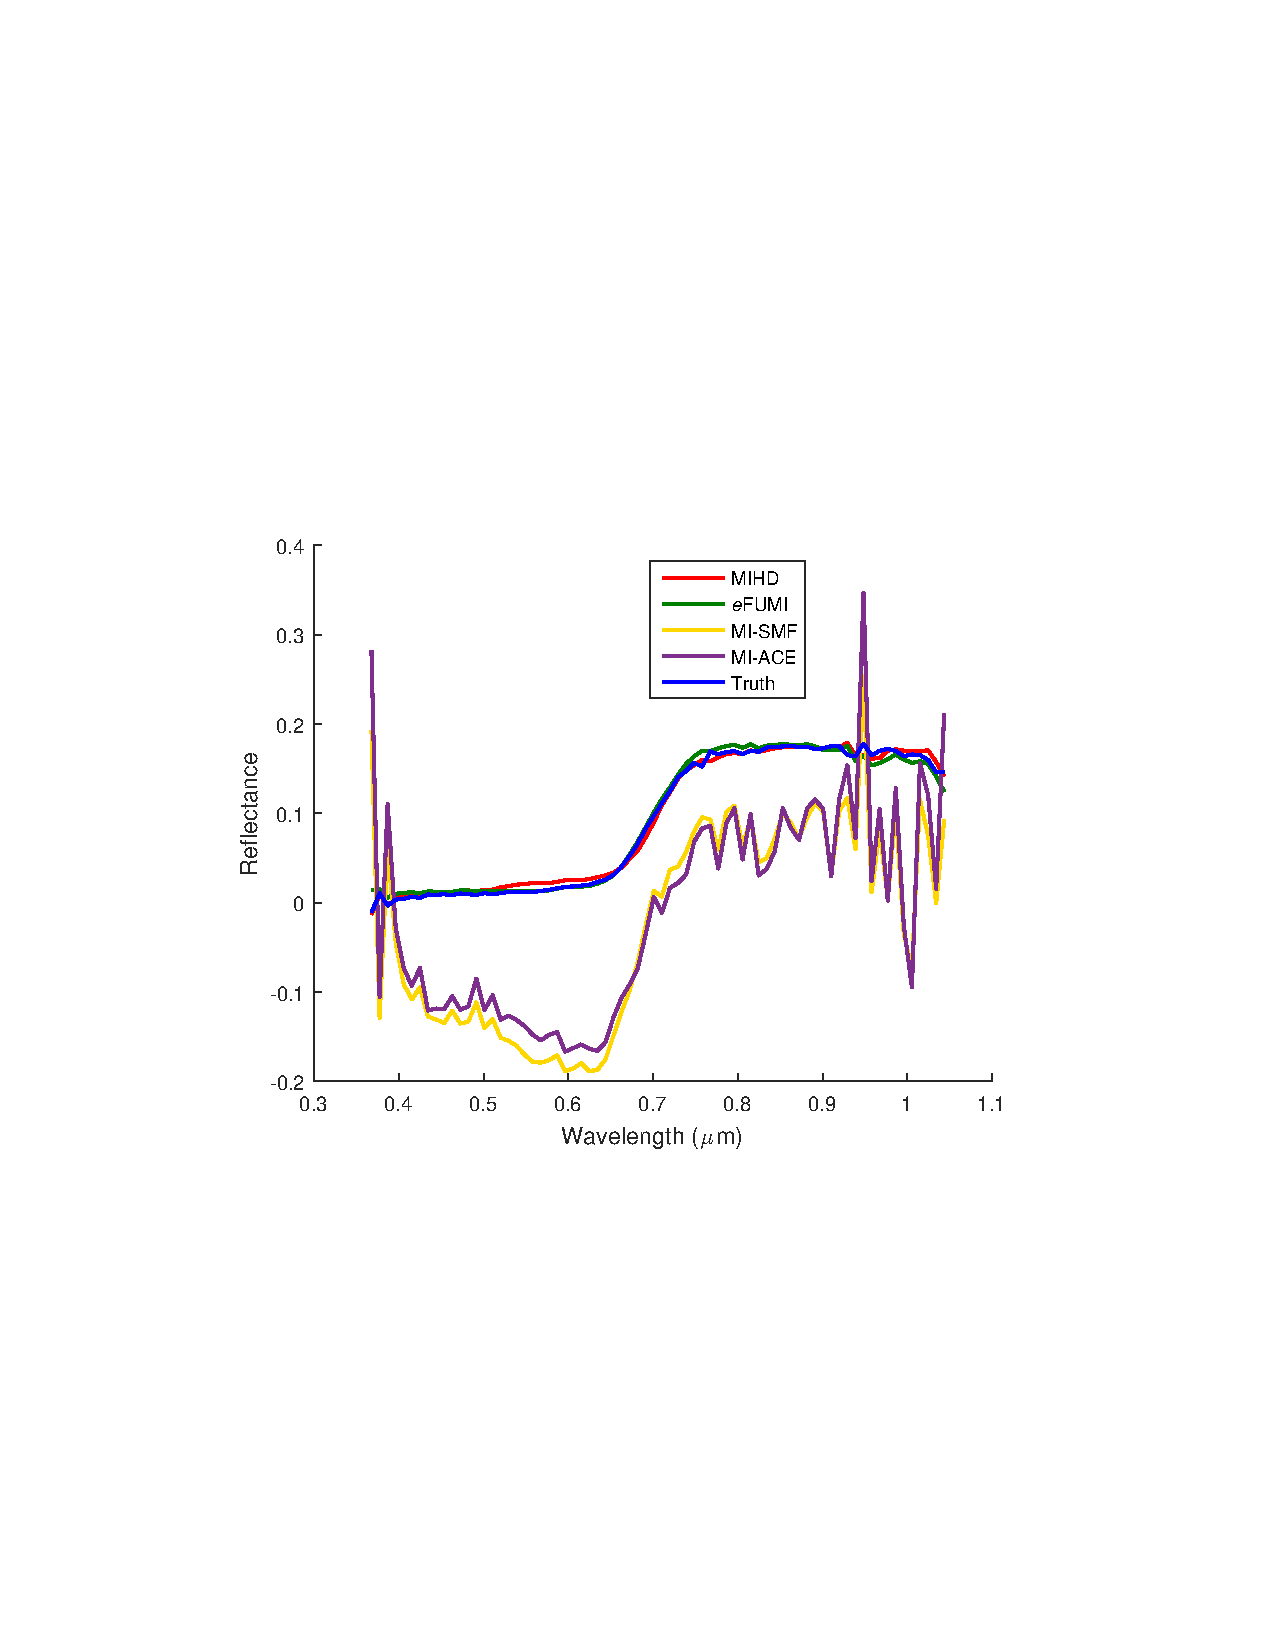
\includegraphics[width=4cm]{gulfport_sigs_brown_train3_test1.pdf} \label{fig:sig_plot_gulfport_brown_train3_test1}}
%		\subfigure[ROC curves]{   
%			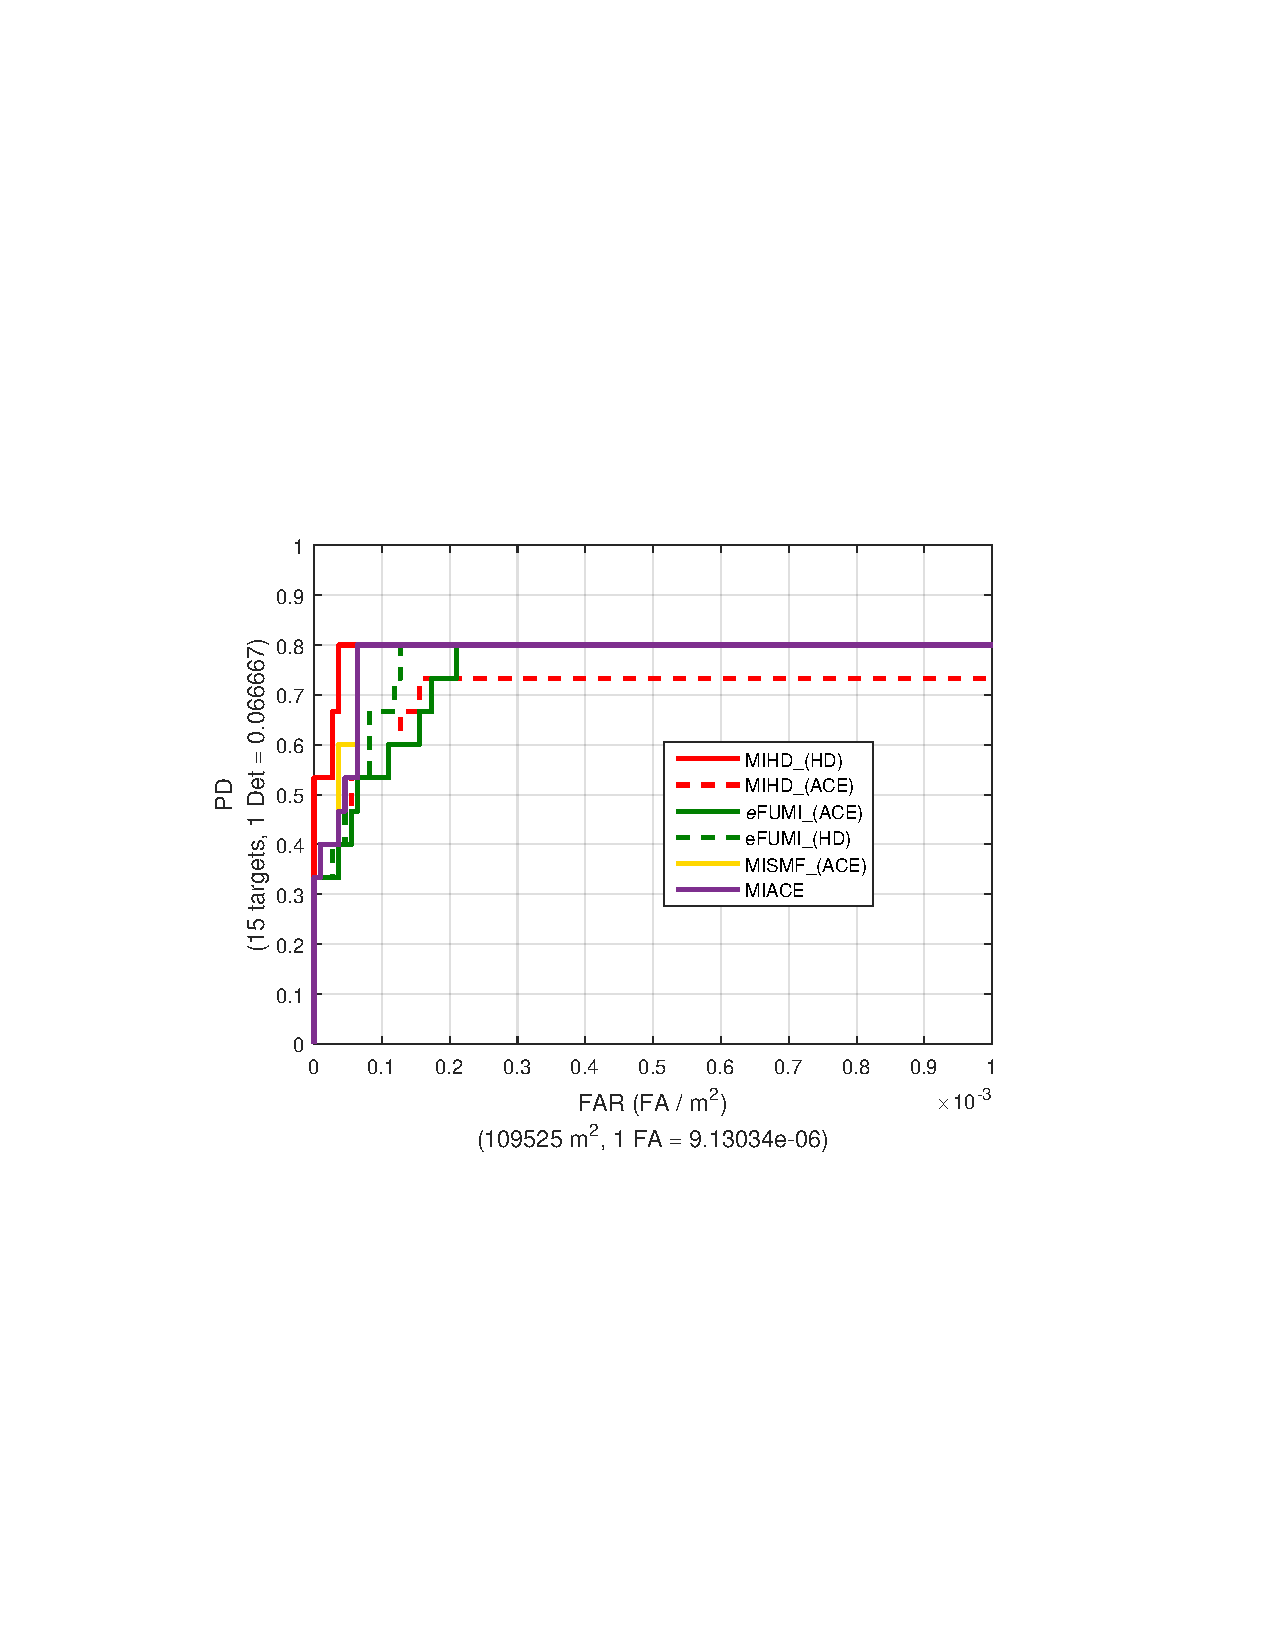
\includegraphics[width=4cm]{gulfport_rocs_brown_train3_test1.pdf} \label{fig:rocs_gulfport_brown_train3_test1}}
%		\caption{Comparison of MI-HE, $e$FUMI, EM-DD and mi-SVM on Gulfport Brown, training on flight 3 testing on flight 1}\label{fig:compare_gulfport_brown_train3_test1}
%	\end{center}
%\end{figure}



%Fig. \ref{fig:compare_gulfport_brown_train1_test3} - \ref{fig:sig_plot_gulfport_brown_train3_test1} and Tab. \ref{tab:AUC_gulfport}  although it does not learn a exact target signature as $e$FUMI. However, MI-HE combined with ACE got very bad detection performance. This indicates that detection method must be consistent with the learning objective. 


	
	
	
	\section{Conclusion and Future Work}
	\label{sec:conclusion}
	
	The proposed MI-HE is able to learn target signature with better quality and achieve competitive and state-of-the-art hyperspectral target detection results when compared to existing multiple instance concept learning methods.
The future work includes optimizing the objective function by quasi-newton method to improve its convergence and adding a discriminative term to promote the discriminativeness of the estimated target signature.
	
	\bibliographystyle{IEEEbib}
	\bibliography{MIHE_IGARSS_ref}
	
\end{document}
